% vim: textwidth=110
% Suppress some acceptable compilation warnings
\RequirePackage[save,showerrors]{silence}
\WarningFilter{transparent}
  {Loading aborted} % Used (or at least tried) by the svg package
\WarningFilter{multicol}
  {May not work with the twocolumn option} % I'm not really using the multicol package
\WarningFilter{latex}
  {Marginpar on page} % Margin stuff moved to not overlap with other stuff, this is fine
\WarningFilter{caption}
  {Unknown document class} % the caption package doesn't know about llncs

% llncs class documentation:
% https://ctan.tetaneutral.net/macros/latex/contrib/llncs/llncsdoc.pdf
\documentclass[dvipsnames]{llncs}

% language settings
\usepackage[main=french,english]{babel}
\newcommand{\en}[1]{\foreignlanguage{english}{\emph{#1}}}
\usepackage{csquotes}
\MakeOuterQuote{"}

% bibliography settings
\usepackage[hyperref=true,backref=true]{biblatex}
\DefineBibliographyExtras{french}{\restorecommand\mkbibnamefamily}
\addbibresource{../references.bib}

% links setup
\usepackage[nobiblatex]{xurl}
\usepackage{hyperref}
\hypersetup{colorlinks=true}

% Hypotheses
\newtheorem{hypo}{Hypothèse}[theorem]

% For file inclusion and figure formatting
\usepackage{caption}
\usepackage{subcaption}

% Other
\usepackage{todonotes}
\usepackage{mathtools}

\title{L'Identification des Projets de Logiciel Libre Accessibles aux Nouveaux Contributeurs}
\author{%
    Premier Auteur\inst{1}%Paul Hervot\inst{1}%
    \and%
    Deuxième Auteur\inst{2}%Benoît Crespin\inst{2}\orcidID{0000-0002-9105-0243}%
}
\institute{Institution du premier auteur \and institution du deuxième auteur} %\institute{EPITA \and Université de Limoge}

\begin{document}
    \maketitle
    \todo{TODO général : réduire à 12 pages}
    \todo{TODO : Ajouter la petite ligne de header (pages paires : nom de la conférence, pages impaires :
    titre court)}
    \todo{TODO : relire le document de référence docx}

    % Abstracts and keywords
    \selectlanguage{french}
    \todo{TODO : réduire à 70-150 mots par abstract}
    \begin{abstract}
        Le logiciel libre prend de plus en plus de place dans le paysage public et industriel, notamment pour
        ses intérêts en terme de transparence des logiciels et de leur gestion démocratique, pour autant le
        simple fait de rendre le code source d'un logiciel publique ne le rend pas automatiquement accessible,
        et les nouveaux contributeurs de ces projets rencontrent de nombreuses barrières d'entrée les
        empêchant parfois de mener leurs contributions à leur terme. Au travers d'une analyse à grande échelle
        de l'archive de Software Heritage, nous testons la pertinence de trois indicateurs dans
        l'identification des projets de logiciel libre accessibles aux nouveaux contributeurs. Nos résultats
        montrent une corrélation positive entre le nombre de contributions menées à leur terme au sein d'un
        projet par de nouveaux contributeurs et la présence d'instructions de contribution, ainsi qu'entre ce
        même nombre et celui des contributeurs uniques récents du projet. De tels indicateurs trouveraient
        leur utilité notamment dans l'enseignement des pratiques du logiciel libre, les enseignants de ce
        sujet ayant souvent du mal à sélectionner des projets accessibles sur lesquels faire travailler les
        étudiants.

        \todo{TODO : utiliser comme mots-clé les catégories de la conférence (pour les deux ou trois
        premiers)}
        \textbf{Mots-clé :} Logiciel libre, Analyse automatique de dépôts logiciels, Barrières d'entrée du
        logiciel libre, Nouveaux contributeurs.
    \end{abstract}
    \selectlanguage{english}
    \begin{abstract}
        Free and Open Source Software make more and more of the public and industrial software landscape,
        notably for its benefits for software transparency and their democratic governance. However, simply
        making the source code of a software public doesn't automatically make it accessible, and new
        contributors approaching these projects often face many barriers to entry that prevent them from
        bringing their contribution to completion. Through a large-scale software mining of the Software
        Heritage archive, we test the pertinence of three signals in the identification of accessible FOSS
        projects for new contributors. Our results show a positive correlation between the number of new
        contributors of a project successfully bringing their contribution to completion and the presence of
        contributing guidelines, as well as between that same number and the number of recent unique
        contributors in the project. Such signals could find a use in the teaching of FOSS practices, as
        teachers of this subject often find it difficult to select an accessible project for their students to
        work on.

        \textbf{Keywords:} FOSS, Mining Software Repositories, Open source barriers to entry, New
        contributors.
    \end{abstract}
    \selectlanguage{french}

    \section{Introduction}

    La pédagogie de projet est une méthode d'enseignement qui consiste à inviter les apprenants à appliquer
    leurs connaissances et à en acquérir de nouvelles au travers d'un projet plus ou moins concret et imitant
    plus ou moins fidèlement une situation réelle. Réalisé soit individuellement soit en groupe, les projets
    aboutissent généralement à une production évaluée par l'enseignant, parfois au travers d'une présentation
    donnée par les apprenants. L'efficacité de cette méthode a fait l'objet de nombreuses recherches au cours
    des années précédentes. Plusieurs méta-analyses concluent que cette méthode a des effets mesurables,
    positifs et importants sur les résultats académiques des apprenants en sciences sociales et en sciences
    naturelles \cite{pbl-2019, pbl-2018}.

    Les projets proposés aux étudiants sont le plus souvent factices, imaginés par les enseignants dans le
    seul but de servir d'exercice. Utiliser au contraire des projets réels, qui ne cessent pas d'exister après
    la fin de la séquence pédagogique, sur lesquels faire travailler les étudiants donne des résultats encore
    meilleurs, mais est aussi plus difficile et incertain à encadrer pour les enseignants \cite{real-pbl-2010,
    real-pbl-2004}. Il est notamment très difficile pour l'enseignant de prévoir à l'avance les problèmes que
    les apprenants risquent de rencontrer, c'est pourquoi d'autres efforts dans cette direction ont tenté un
    compromis, consistant à créer des projets de logiciel libre aussi proches des situations réelles que
    possible, mais dédiés à l'éducation \cite{oss-edu-2008}. Les projets en question ne sont cependant plus
    accessibles aujourd'hui, une explication possible à leur disparition étant leur portée réduite à
    l'éducation et l'absence d'une communauté persistante autour d'eux.

    Bien qu'elles soient plutôt rares, quelques initiatives existent aussi pour enseigner spécifiquement les
    pratiques du logiciel libre dans l'éducation supérieur et la formation tout au long de la vie. Certaines
    sont des initiatives venant des communautés du logiciel libre, comme le
    \href{https://www.edx.org/professional-certificate/linuxfoundationx-open-source-software-development-linux-and-git}{\en{Professional
    Certificate in Open Source Software Development, Linux and Git}} de la \en{Linux Foundation}, et en
    particulier la première séquence :
    \href{https://www.edx.org/course/open-source-software-development-linux-for-developers}{\en{Open Source
    Software Development: Linux for Developers}} ou les séminaires de
    l'\href{https://opensource.org/osi-open-source-education}{\en{open source initiative}}. Enfin, certaines
    universités proposent des cursus en informatique ayant des éléments visant spécifiquement les pratiques du
    logiciel libre, c'est le cas notamment de l'Université de l'État de Caroline du Nord aux États-Unis, qui a
    expérimenté plusieurs façons d'inclure la contribution aux projets de logiciel libre dans leurs cursus
    d'informatique \cite{oss-edu-2008, oss-edu-2007} ; mais aussi de l'université de Calais qui propose
    actuellement un
    \href{https://www.univ-littoral.fr/formation/offre-de-formation/masters/master-informatique-ingenierie-du-logiciel-libre/}{Master
    Informatique - Ingénierie du logiciel libre}, sous la forme d'une formation en alternance.

    \section{Les nouveaux contributeurs dans le logiciel libre}

    \textcite{barriers-2018} notent la difficulté des nouveaux volontaires à rejoindre une communauté de
    logiciel libre, citant comme exemple extrême le projet Apache Hadoop qui a vu 82\% de ses nouveaux
    volontaires quitter le projet après leur première contribution \parencite{hadoop-dropout-2013}. Une des
    tendances qu'ils trouvent est que la majorité ($58\%$) des barrières rencontrées dans leur étude sont de
    nature sociale ("\en{community-oriented}") et non techniques \parencite[p.~1008]{barriers-2018}.
    Concernant les aspects plus techniques, il semble que les outils et la documentation représentent la
    majorité des barrières rencontrées, alors même que ces éléments ont spécifiquement pour objectif d'aider
    les nouvelles contributions. C'est un type de barrière qui semble amplifié lorsque les méthodes
    d'apprentissage et de traitement de l'information de la personne consistent à rassembler le plus
    d'information possible avant de commencer à agir. Ces méthodes étant sur-représentées chez les femmes
    \parencite{gender-information-processing-1995,gender-information-processing-2015}, ces barrières
    deviennent discriminantes selon le genre, et peuvent potentiellement participer à expliquer la
    sous-représentation des femmes dans les communautés de logiciel libre.

    \label{sec:accessibility-measure}
    Plusieurs essais de mesure \emph{a posteriori} de l'accessibilité des projets de logiciel libre on eu
    lieu, en majorité de façon qualitative
    \parencites{newcomers-accessibility-2016}{newcomers-onboarding-2018}[voir
    aussi][]{newcomers-adaptation-2005}. Une autre approche, plus quantitatives, consiste à compter
    automatiquement le nombre de contributeurs accumulés depuis le début de la vie du projet et jusqu'à
    différents points dans le temps, afin d'étudier la progression de ce nombre\cite{contributor-count-2006}.

    \textcite{signals-2019} traitent d'une question similaire en essayant de déterminer quels sont les signaux
    que les potentiels nouveaux contributeurs regardent (et comment) pour choisir un projet de logiciel libre
    auquel contribuer. Ils s'intéressent pour cela spécifiquement aux projets disponibles publiquement sur
    \en{github}, ce qui leur permet, après une approche exploratoire pour dégager des hypothèses, d'étudier
    empiriquement l'effet des signaux que la plateforme met en évidence.

    \textcite{signals-2019} suggèrent qu'une mesure possible de l'accessibilité pour les nouveaux
    contributeurs ("\en{newcomers openness}" dans l'article) est le pourcentage de \en{pull requests} créées
    par des contributeurs externes. Ils définissent les contributeurs externes par opposition aux
    contributeurs principaux ("\en{core contributors}") qu'ils identifient, eux, comme étant les personnes
    auteurs de plus de 5\% des \en{commits} du projet. En réalité cependant, leur étude quantitative simplifie
    la mesure en ne retenant que la présence ou non de \en{pull request} venant de nouveaux contributeurs
    (p.~16), ce qui leur permet de n'étudier qu'une variable binaire.

    \section{L'analyse automatique ("minage") de projets de logiciel libre}
    \todo{TODO : fusionner les sections 2 et 3}

    Pour leur analyse quantitative, \textcite{signals-2019} commencent par collecter des données sur la
    plateforme d'hébergement de code source \en{github} via son \en{API}. Ce choix est cohérent avec un grand
    nombre d'études de ces dernières années \parencite{github-mapping-2017}, la plateforme est très populaire
    dans le milieu du logiciel libre et a connu une croissance très importante ces dernières années. Ces mêmes
    études notent cependant parfois que se restreindre à cette seule plateforme est une limite diminuant la
    représentativité de l'échantillon qu'elles étudient \parencite{swh-growth-2019}. Les limites et erreurs
    courantes liées au minage de \en{github} font d'ailleurs l'objet d'une littérature grandissante et
    remettant potentiellement en question les résultats des études utilisant cette technique sans détailler
    suffisamment leur méthodologie de collecte des données \parencite{mining-github-2014,penumbra-oss-2022}.

    Le nombre de projets et d'artéfacts qui leur sont lié est par ailleurs en augmentation rapide, voir
    exponentielle. \textcite{swh-growth-2019} estiment que le nombre de \en{commits} uniques originaux double
    environ tous les trente mois, le nombre de fichiers uniques originaux doublerait quant à lui tous les
    vingt-deux mois. Cette explosion du nombre de \en{commits} et de fichiers s'accompagne d'un important
    phénomène de duplication : de nombreux fichiers se retrouvent dans de nombreux projets différents, comme
    les notices de licence par exemple. Les \en{commits} eux-même peuvent se trouver dans plusieurs projets
    différents, c'est ce qui arrive lorsqu'un projet débute en tant que \en{fork} d'un autre. Ces deux points
    rendent de plus en plus difficile l'analyse efficace et à grande échelle de l'historique de développement
    des projets de logiciel libre.

    \subsection{L'archive de logiciels de Software Heritage}

    \label{ssec:swh-graph}

    Les techniques de compression de graphe sont aujourd'hui suffisamment avancées pour permettre une nouvelle
    approche à cette analyse automatique des projets, en rendant un très grand nombre de ceux-ci disponibles
    au sein d'une même structure de donnée unifiée et optimisée \parencite{swh-graph-2020}. Cette approche
    permet par exemple de grandement faciliter la détection des \en{clones} ou \en{forks} de projets, c'est à
    dire des projets ayant une part de leur historique de développement en commun. La structure de donnée
    proposée par \textcite{swh-graph-2020} est un graphe orienté où chaque \en{commit} est représenté par un
    nœud et où chaque arc $u \xrightarrow{succ} v$ ("$v$ est un successeur de $u$", autrement dit pour les
    \en{commits} "$v$ est un ancêtre immédiat de $u$") possède aussi un arc inverse $u \xleftarrow{pred} v$
    ("$u$ est un prédécesseur de $v$"). Une telle structure permet donc de trouver tous les \en{fork} d'un
    projet avec un classique calcul de composante fortement connexe, ce qui peut se faire avec un simple
    parcours profondeur ou largeur du graphe à partir de n'importe lequel de ses \en{commits}.

    Software Heritage est une initiative exploitant ces techniques de compression afin de construire une
    archive aussi complète que possible du code source actuellement disponible publiquement dans le monde.
    L'archive est elle aussi publique et un de leurs objectifs est de la rendre exploitable pour la recherche
    \parencite{swh-2017}. Il s'agit du corpus que \textcite{swh-graph-2020} ont utilisé comme exemple pour
    leur modèle de compression. L'archive comptait en 2018 plus d'un milliard de \en{commits} uniques archivés
    depuis quatre-vingt-cinq millions d'origines différentes (telles que des \en{remotes} \en{git} ou des
    versions de paquets Python publiés sur \href{https://pypi.org/}{PyPi}). L'archive est stockée dans une
    structure en ajout seul : elle grandit de façon continue en archivant petit à petit de nouveaux projets
    et en ajoutant de nouveaux artéfacts à chaque évolution des projets déjà archivés, ce qui en fait l'un des
    corpus les plus complets et exploitable par la recherche scientifique
    \parencite{swh-2019,swh-growth-2019}.

    \subsection{Sélection des projets étudiés}

    Dans une méta-analyse concernant l'étude des barrières d'entrée, \textcite{barriers-meta-2015} remarquent
    un biais courant dans la sélection des projets de logiciel libre retenus dans la littérature (p. 83) : les
    auteurs ont tendance à plutôt étudier les projets importants, matures et populaires, car ils sont plus
    susceptibles d'apporter un volume important de données. Bien que les résultats semblent cohérent avec les
    plus rares études sélectionnant de petits projets, ils invitent la communauté scientifique à s'y
    intéresser plus en profondeur et à constituer des échantillons plus variés.

    Quand \textcite{mining-github-2014} analysent les \en{pull requests} sur \en{github}, ils ne retiennent
    que les projets ayant au moins deux auteurs de \en{commits} uniques, ce qu'ils considèrent comme des
    projets vraiment collaboratifs. Ce choix vient de leur observation qu'une très grande partie des projets
    hébergés sur la plateforme ($71\%$) sont des projets personnels, utilisés par leurs auteurs à des fins
    d'expérimentation ou de stockage, sans réelle ouverture à la collaboration.

    \section{Méthodologie}

    \subsection{Problématique}

    La question de l'accessibilité des projets de logiciel libre pour les nouveaux contributeurs est encore
    assez peu explorée de façon quantitative dans la littérature. \textcite{signals-2019} se sont intéressés
    aux signaux que les potentiels nouveaux contributeurs utilisent afin de sélectionner les projets auxquels
    ils \emph{essayent} de contribuer, c'est à dire les signaux formant l'attractivité de ces projets. Nous
    nous attacherons ici à déterminer si certains de ces mêmes signaux sont, de surcroit, prédictifs d'une
    réelle accessibilité de ces projets, c'est à dire à quel point de nouveaux contributeurs
    \emph{réussissent} à produire une contribution apparaissant dans l'historique de développement du projet.

    Comme nous l'avons vu, la recherche quantitative portant sur les historiques de développement des
    logiciels libre a récemment eu tendance à limiter sa population étudiée aux projets hébergés sur la
    plateforme \en{github}, ce qui occulte une part importante des projets de logiciel libre
    \parencites{mining-github-2014}{penumbra-oss-2022}. Pour améliorer la représentativité de nos résultats,
    nous utiliserons donc dans notre étude l'archive de Software Heritage, celle-ci ne se limitant pas aux
    projets hébergés sur \en{github}, ni même au système de versionnement \en{git}.

    L'usage de cette archive nous limitera en revanche dans le type de données que nous pourrons collecter. Il
    sera par exemple impossible de mesurer le nombre d'\en{issues} publiées par de nouveaux intervenants dans
    le \en{bug tracker} des projets, ou le nombre de \en{pull requests}. Nous devrons nous servir
    exclusivement des données disponibles dans l'historique de développement en tant que tel, comme l'ensemble
    des \en{commits}, leurs auteurs, leur date, ainsi que les noms et contenus des fichiers qu'ils manipulent.

    \subsection{Mesure de l'accessibilité choisie}

    La variable mesurée qui sera utilisée comme proxy pour l'accessibilité d'un projet pour les nouveaux
    contributeurs est le nombre de contributeurs apparaissant pour la première fois dans l'historique de
    développement du projet au cours de la période de référence étudiée : du premier juin 2019 au premier
    septembre 2019 \parencite[voir section \ref{sec:accessibility-measure}, ainsi
    que][p.~13,16]{signals-2019}. Cette période de référence a été choisie sur recommandation de Software
    Heritage, la désignant comme un bon compromis entre le nombre de projets pour lesquels les données sont
    disponible dans l'archive à cette période et le caractère récent des observations.

    \subsection{Hypothèses}

    \newcommand{\newhyp}[2]{%
        \begin{hypo}
            \label{hyp:#1}#2
        \end{hypo}%
    }

    \newhyp{contributionguidelines}{%
        les projets possédant des instructions de contribution (fichier type \texttt{CONTRIBUTING.md} ou
        section type \en{Contributing} dans un fichier type \texttt{README.md}) sont plus accessibles pour
        les nouveaux contributeurs que ceux n'en ayant pas \parencite[voir][p.~11]{signals-2019}.%
    }

    \newhyp{recentcontributorcount}{%
        le nombre de contributeurs uniques récents (au cours des six mois précédents la période de référence
        étudiée) d'un projet est positivement corrélée à son accessibilité pour les nouveaux contributeurs
        \parencite[voir][p.~12-13,16]{signals-2019}.%
    }

    \newhyp{recentcommitcount}{%
        le nombre de \en{commits} récents (au cours des six mois précédents la période de référence étudiée)
        au sein d'un projet est positivement corrélé à son accessibilité pour les nouveaux contributeurs
        \parencite[voir][p.~13,16]{signals-2019}.
    }

    \subsection{Constitution de l'échantillon}
    \label{sec:constitution_echantillon}

    L'échantillon de départ est constitué de la totalité des projets archivés dans le graphe de Software
    Heritage. Plusieurs critères d'exclusion ont ensuite été appliqués :

    \begin{itemize}
        \item quand deux projets ou plus ont un ou plusieurs \en{commits} en commun et sont donc des
            \en{forks} les uns des autres, seul celui qui a reçu le plus d'activité (mesuré par le nombre
            d'arêtes maximal entre le \en{commit} source et un des \en{commits} initiaux) a été retenu comme
            représentant du groupe, afin d'éviter de compter plusieurs fois les mêmes historiques ;
        \item les projets n'ayant enregistré aucune activité (aucun \en{commit}) au cours de la période de
            référence étudiée sont considérés inactifs et n'ont pas été retenus
            \parencite[voir][]{mining-github-2014} ;
        \item les projets ayant vu moins de deux contributeurs uniques récents (au cours des six mois
            précédent la période de référence) sont considérés comme des projets individuels, non réellement
            collaboratifs et n'ont pas été retenus \parencite[voir][]{mining-github-2014}.
    \end{itemize}

    \subsection{Collecte initiale des données}

    \todo{TODO : il y a peut être des explications à dédupliquer avec la section \ref{ssec:swh-graph}}
    Comme présenté en section \ref{ssec:swh-graph}, l'archive de Software Heritage se présente sous la forme
    d'un graphe orienté. Ses nœuds représentent diverses entités de l'historique de développement, parmi
    lesquelles les \en{commits} (appelés \en{revisions} au sein du graphe), les origines (l'URL à partir de
    laquelle a été archivé un projet), les \en{snapshots} (point de départ d'un archivage précis et daté,
    beaucoup de projets étant ré-archivés régulièrement), les dossiers et les fichiers (contenu du projet). Un
    arc $u \xrightarrow{succ} v$ peut donc signifier, en fonction des types de $u$ et $v$ : 

    \begin{itemize}
        \item que $u$ est un \en{commit} créé immédiatement après le \en{commit} $v$ ;
        \item que $v$ est un archivage (\en{snapshot}) du projet disponible à l'origine $u$ ;
        \item que $v$ est le dernier \en{commit} d'une des branches visibles lors de l'archivage
            (\en{snapshot}) $u$ ;
        \item que $v$ est le dossier racine du contenu du projet en l'état du \en{commit} $u$ ;
        \item etc.
    \end{itemize}

    Afin de découvrir et sélectionner les projets dans lesquels nous collecterons les données, une première
    exploration est lancée à partir de chaque nœud de type \en{origin} du graphe avec deux objectifs :
    identifier tous les \en{forks} du projet de départ et sélectionner un représentant pour le groupe. Pour ce
    faire, l'exploration prend la forme d'un premier parcours largeur sur les arcs \en{successor} des nœuds
    \en{revision} afin d'identifier tous les \en{commits} initiaux accessibles depuis l'origine de départ, puis
    d'un deuxième parcours largeur partant de chacun de ces \en{commits} initiaux afin d'identifier tous les
    autres nœuds \en{origin} de la composante connexe. Des marqueurs de niveaux lors de ce deuxième parcours
    largeur permettent de mesurer la distance qui éloigne chaque origine ainsi découverte de son \en{commit}
    initial le plus éloigné. Pour chaque composante connexe, seule le \en{snapshot} le plus récent de
    l'origine la plus éloignée d'un \en{commit} initial est retenu pour la collecte.

    Pour tous les projets ainsi retenu, un nouveau parcours largeur est démarré à partir de sa branche
    principale afin de récolter les données de recherche. Le nombre de contributeurs uniques récents et de
    \en{commits} récents se compte facilement en accédant à la date et aux auteurs de chaque nœud
    \en{revision} rencontré, mais la vérification de la présence d'instructions de contribution demande un peu
    plus de travail. Le graphe possède le nom et la hiérarchie de chacun des fichiers du projet pour chaque
    \en{commit}, mais pas leur contenu. Ce parcours se contente donc initialement de vérifier la présence d'un
    fichier nommé \texttt{CONTRIBUTING.md} ou assimilé, nous considérons que le projet possède effectivement
    des instructions de contribution si un tel fichier existe. Si aucun fichier de ce type n'est trouvé, nous
    recherchons alors la présence d'un fichier nommé \texttt{README.md} ou assimilé, l'absence d'un tel
    fichier nous permet de conclure que le projet ne possède \emph{pas} d'instructions de contribution. Si un
    tel fichier est trouvé, en revanche, nous devons vérifier son contenu avant de conclure, nous sauvegardons
    alors l'identifiant unique du contenu du fichier afin de pouvoir l'analyser lors d'une phase de collecte
    ultérieure. Enfin, le nombre de nouveaux contributeurs est calculé en comptant les contributeurs uniques
    de la période de référence qui n'apparaissent dans aucun \en{commit} antérieur à cette période (et non
    seulement au cours des six mois précédents la période de référence).

    \subsection{Collecte complémentaire des données}
    \label{sec:collectreadme}

    Il nous faut maintenant vérifier le contenu du fichier \texttt{README.md} (ou assimilé) retenu pour chaque
    projet ne possédant pas de fichier \texttt{CONTRIBUTING.md} (ou assimilé) afin de déterminer s'ils
    possèdent ou non des instructions de contribution, et ainsi compléter notre jeu de donnée. Le contenu des
    fichiers est bien archivé par Software Heritage mais n'est pas disponible directement dans le graphe, il
    est en revanche possible de télécharger ces contenus de deux autres façons différentes : soit via des
    requêtes HTTP sur le site web \href{https://archive.softwareheritage.org/}{archive.softwareheritage.org},
    accessible publiquement, soit en téléchargeant les contenus directement depuis leur \en{registry} Amazon
    S3 (\href{https://registry.opendata.aws/software-heritage}{registry.opendata.aws/software-heritage}), lui
    aussi accessible publiquement. Le site limite le nombre de requêtes autorisées par adresse IP à quelques
    dizaines par heure. Le \en{registry} n'impose pas ce genre de limite, mais le contenus de certains
    fichiers n'y est pas encore disponible. Nous utiliserons donc en priorité le \en{registry} Amazon S3 pour
    télécharger le contenu des fichiers \texttt{README} nécessaires, puis le site pour tous ceux que nous ne
    parviendrons pas à y trouver.

    Une fois le contenu des \texttt{README} téléchargés, nous y cherchons une section dont le nom contient le
    mot \en{contributing} ou un mot proche. Pour identifier les noms de section dans les fichiers téléchargés,
    nous supposons que ceux-ci sont formatés suivant un des deux standards les plus répandus de formatage de
    text brut : le Markdown (dont l'extension courante est \texttt{.md}) ou le reStructuredText (dont
    l'extension courante est \texttt{.rst}). Le format Markdown autorise deux façon de définir une section
    \parencite{markdown-headings}, la première consiste à démarrer une ligne avec un ou plusieurs caractères
    \texttt{\#} puis d'écrire le nom de la section sur la fin de la ligne, l'autre consiste à écrire
    directement le nom de la section, puis à la "souligner" en écrivant plusieurs fois le caractère \texttt{=}
    ou \texttt{-} sur la ligne suivante. Le format reStructuredText n'autorise qu'une seule façon de définir
    des sections, en soulignant une ligne de la même façon que la deuxième méthode du Markdown, à ceci près
    que d'autres caractères sont aussi acceptés pour composer la ligne \parencite{rst-sections}.

    Pour déterminer si un fichier \texttt{README} contient des instructions de contribution, nous identifions
    donc tous les noms de section le composant et vérifions si l'un d'eux contient le mot \en{contributing} ou
    assimilé.

    \subsection{Reproduction des travaux}

    \todo{TODO : anonymiser, voir ne pas mentionner, possibilité d'en refaire un anonyme}
    Afin d'améliorer la transparence méthodologique de ce travail et d'aider l'éventuelle reproduction des
    résultats qui y sont présentés, un \en{replication package} contenant le code source et les bibliothèques
    utilisés dans ce mémoire, ainsi que les données brut collectées, a été publié sur Zenodo
    \parencite{replication-package}.

    \section{Résultats et discussion}

    % Figure caption setup
    \captionsetup[figure]{format=plain,singlelinecheck=true,justification=centering}
    \captionsetup[subfigure]{format=plain,singlelinecheck=true,justification=centering}
    \captionsetup[table]{format=plain,singlelinecheck=true,justification=centering}

    L'analyse du graphe de Software Heritage a permis de déterminer les quatre variables de recherche pour
    $60 966$ projets distincts dont les historique de développement sont eux aussi entièrement distincts deux
    à deux (aucun projet analysé n'est un \en{fork} d'un autre).

    \subsection{Forme et distribution des données collectées}

    \begin{table}[ht]
        \centering
        \begin{tabular}{c|c}
            \begin{tabular}{ll}
 & hasContrib \\
count & 27619 \\
unique & 2 \\
top & no \\
freq & 23740 \\
\end{tabular}
 &
            \begin{tabular}{lr}
 & \textbf{recentCommitCount} \\
count & 60966.00 \\
mean & 61.79 \\
std & 408.96 \\
min & 2.00 \\
25\% & 8.00 \\
50\% & 19.00 \\
75\% & 49.00 \\
max & 36176.00 \\
\end{tabular}
\\
            \hline
            \\
            \begin{tabular}{lr}
 & \textbf{recentContributorCount} \\
count & 60966.000000 \\
mean & 3.246268 \\
std & 6.983897 \\
min & 2.000000 \\
25\% & 2.000000 \\
50\% & 2.000000 \\
75\% & 3.000000 \\
max & 688.000000 \\
\end{tabular}
 &
            \begin{tabular}{lr}
 & newContributorCount \\
count & 60966.000000 \\
mean & 0.522209 \\
std & 1.663200 \\
min & 0.000000 \\
25\% & 0.000000 \\
50\% & 0.000000 \\
75\% & 1.000000 \\
max & 130.000000 \\
\end{tabular}

        \end{tabular}
        \caption{Aperçu statistique des données collectées}
        \label{tab:data_description}
    \end{table}
    \todo{TODO : mettre les noms de propriété en gras (hasContrib, recentCommitCount, etc.)}

    Un aperçu initial des données collectées (table~\ref{tab:data_description}) révèle quelques propriétés
    intéressantes de la population étudiée. Les projets possédant des instructions de contribution sont
    significativement moins nombreux ($8 572$, soit environ $14\%$ des projets) que ceux n'en possédant pas.
    L'écart entre la moyenne et la médiane du nombre de \en{commits} récents, ainsi que sont écart type,
    indiquent une forte variation de ce nombre au sein de la population étudiée, mais aussi la présence de
    quelques individus extrêmes, avec un maximum à $36 176$ \en{commits} récents observés dans un seul projet.
    Cette dernière observation se retrouve aussi dans le nombre de contributeurs récents, bien que de façon
    moins spectaculaire. Rappelons à la vue des quantiles de cette dernière valeur que les projets ayant vu
    moins de deux contributeurs distincts récents ont été exclus de l'étude (voir section
    \ref{sec:constitution_echantillon}), ce qui explique que la valeur minimale soit de deux.

    \begin{figure}[ht]
        \begin{subfigure}[t]{0.3\textwidth}
            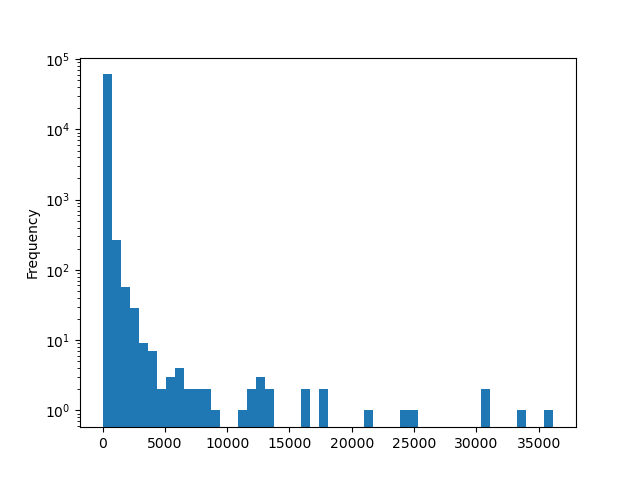
\includegraphics[width=\textwidth]{../experiment/data_analysis/recentCommitCount_distribution}
            \caption{Nombre de \emph{commits} récents\\(ordonnées logarithmiques)}
        \end{subfigure}
        \begin{subfigure}[t]{0.3\textwidth}
            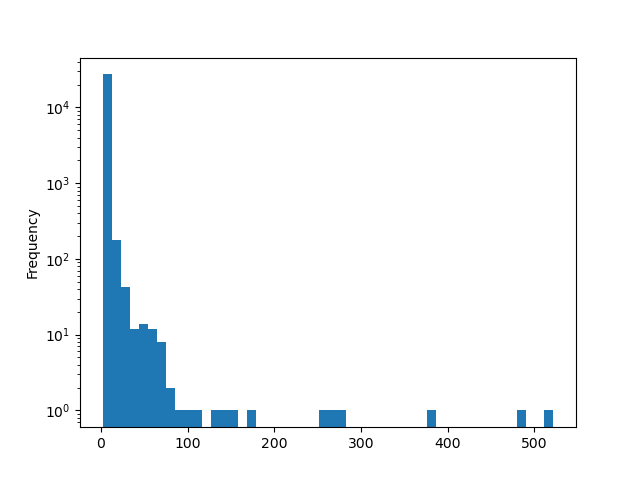
\includegraphics[width=\textwidth]{../experiment/data_analysis/recentContributorCount_distribution}
            \caption{Nombre de contributeurs récents\\(ordonnées logarithmiques)}
        \end{subfigure}%
        \begin{subfigure}[t]{0.3\textwidth}
            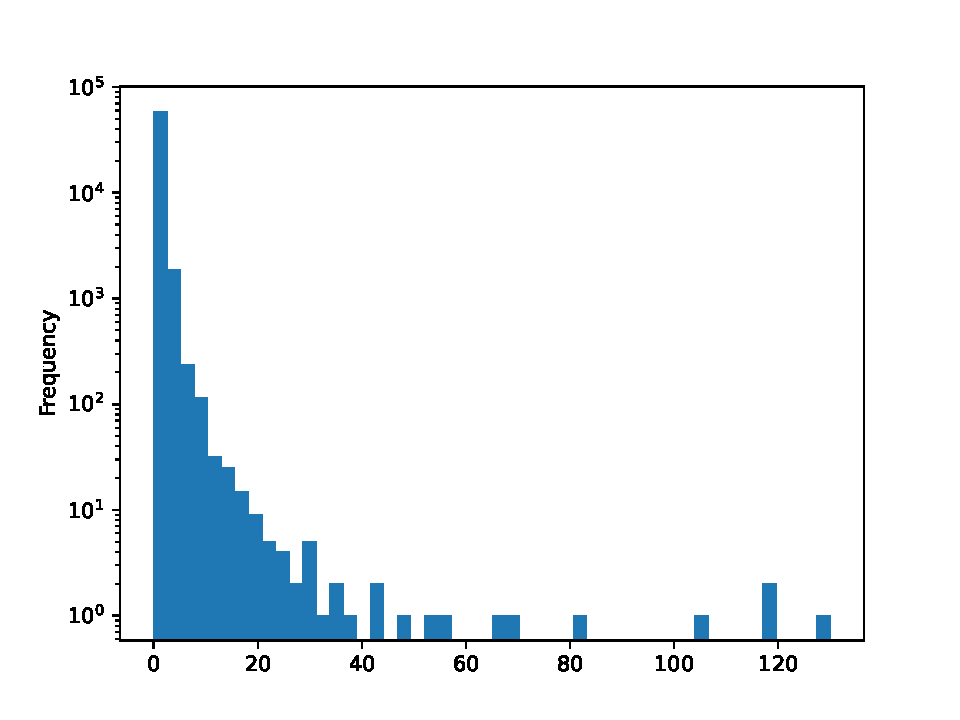
\includegraphics[width=\textwidth]{../experiment/data_analysis/newContributorCount_distribution}
            \caption{Nombre de nouveaux contributeurs\\(ordonnées logarithmiques)}
        \end{subfigure}

        \caption{Distribution des individus selon chaque variable numérique}
        \label{fig:distribution}
    \end{figure}
    \todo{TODO : voir à augmenter la taille des légendes dans les graphiques pour améliorer la lisibilité}
    \todo{TODO : repasser les bar plots en vectoriel, mais pdf et pas svg}

    \begin{figure}[ht]
        \begin{subfigure}[t]{0.3\textwidth}
            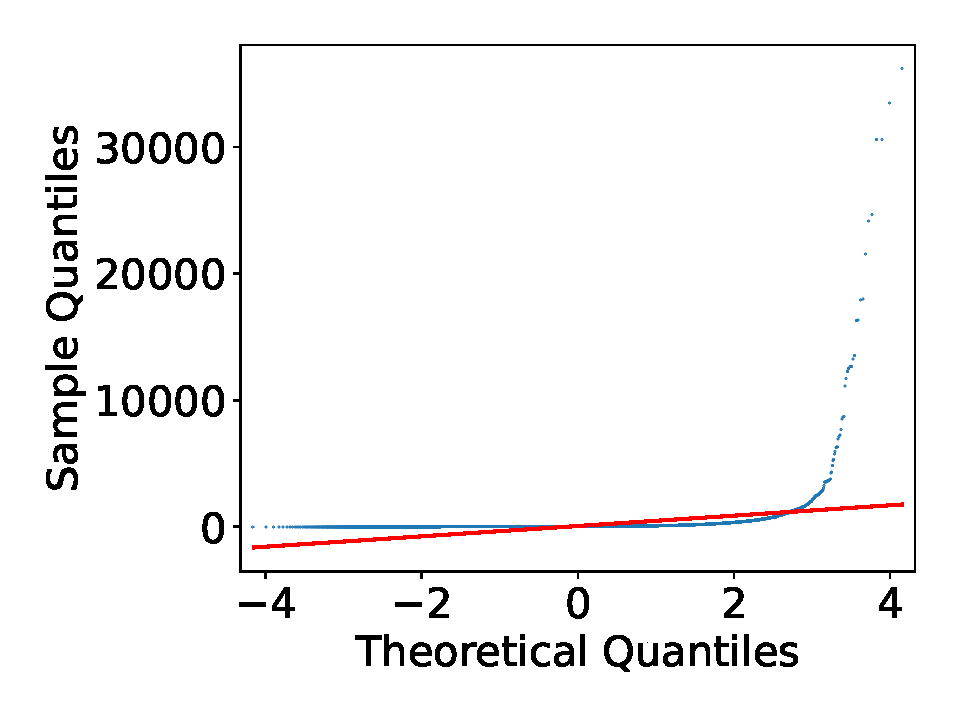
\includegraphics[width=\textwidth]{../experiment/data_analysis/recentCommitCount_qqplot}
            \caption{Nombre de \emph{commits} récents}
        \end{subfigure}
        \begin{subfigure}[t]{0.3\textwidth}
            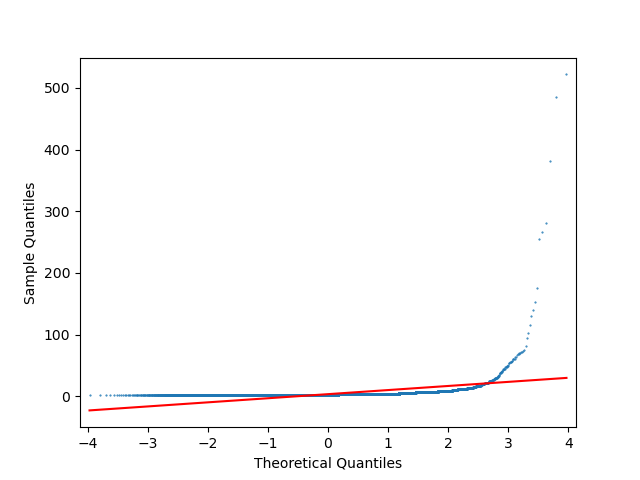
\includegraphics[width=\textwidth]{../experiment/data_analysis/recentContributorCount_qqplot}
            \caption{Nombre de contributeurs récents}
        \end{subfigure}%
        \begin{subfigure}[t]{0.3\textwidth}
            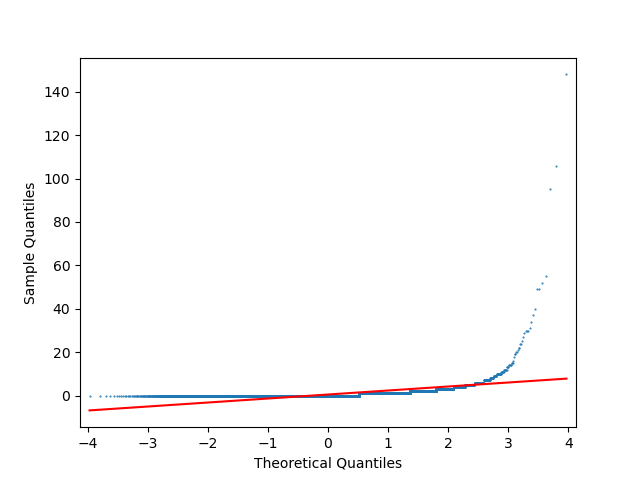
\includegraphics[width=\textwidth]{../experiment/data_analysis/newContributorCount_qqplot}
            \caption{Nombre de nouveaux contributeurs}
            \label{sfig:newContributorQQplot}
        \end{subfigure}

        \caption{Diagrammes quantile-quantile pour chaque valeur numérique}
        \label{fig:qqplots}
    \end{figure}

    Une visualisation de la distribution de la population selon chaque variable numérique
    (Fig.~\ref{fig:distribution}) semble donner une forme d'exponentielle décroissante pour chacune d'elles,
    ce qui signifie par exemple que les projets ayant peu de nouveaux contributeurs sont les plus courants,
    alors que ceux en ayant plus deviennent rapidement beaucoup plus rare à mesure que le nombre augmente. Les
    diagrammes quantile-quantile (Fig.~\ref{fig:qqplots}) de ces variables confirment de façon un peu plus
    formelle que leur distribution ne suit pas une loi normale, ce qui sera important pour l'interprétation
    des modèles obtenus plus loin dans cette analyse.

    \subsection{Lien entre la présence d'instructions de contribution et le nombre de nouveaux contributeurs}

    \begin{figure}[ht]
        \begin{subfigure}[t]{0.5\textwidth}
            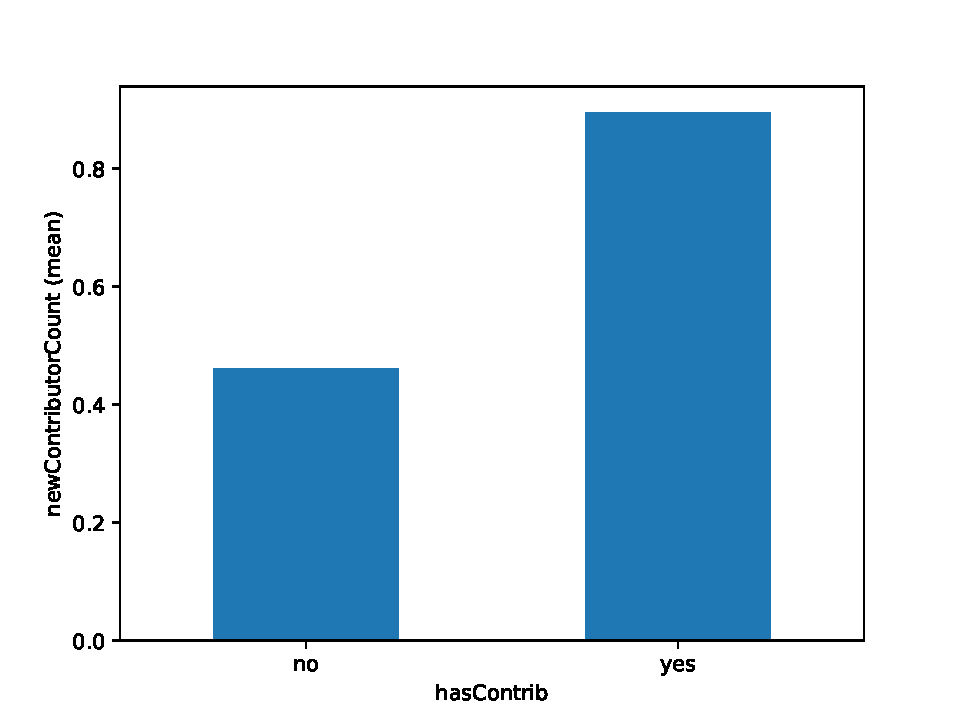
\includegraphics[width=\textwidth]{../experiment/data_analysis/hasContrib_meanNewContributorCount}
            \caption{Moyenne du nombre de nouveaux contributeurs pour chaque catégorie}
        \end{subfigure}%
        \begin{subfigure}[t]{0.5\textwidth}
            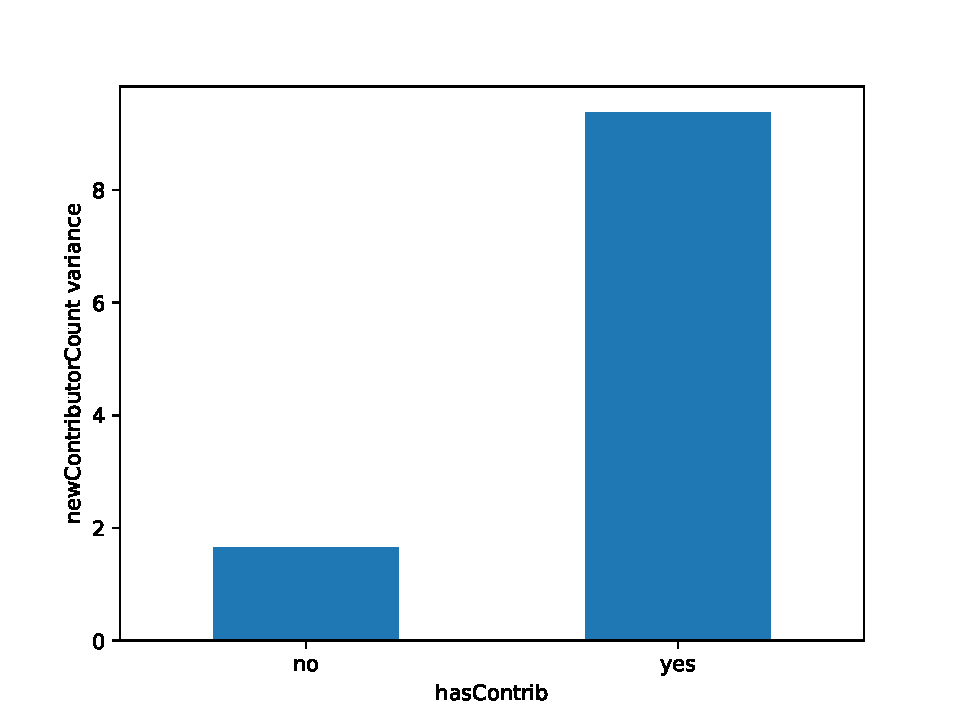
\includegraphics[width=\textwidth]{../experiment/data_analysis/hasContrib_varianceNewContributorCount}
            \caption{Variance du nombre de nouveaux contributeurs pour chaque catégorie}
            \label{sfig:hasContribVariance}
        \end{subfigure}

        Mann-Whitney statistic: $U = 52115090$ ($p = 1.783731 \times 10^{-60}$, $ρ = 0.56593036$)
        \caption{Moyenne du nombre de nouveaux contributeurs pour chaque catégorie}
        \label{fig:hasContrib}
    \end{figure}

    La figure \ref{fig:hasContrib} montre la moyenne du nombre de nouveaux contributeurs au sein des projets
    possédant des instructions de contribution d'une part, et ceux n'en possédant pas d'autre part.

    Ces deux catégories de projets ont été comparées avec un test de Wilcoxon-Mann-Whitney. Celui-ci donne une
    taille d'effet $ρ \approx 0.57$, ce qui signifie en langage courant que si l'on choisi au hasard un projet
    $A$ possédant des instructions de contribution et un projet $B$ n'en possédant pas, il y a environ $57\%$
    de chances que le projet $A$ ait vu un plus grand nombre de nouveaux contributeurs durant la période
    étudiée que le projet $B$. Le test confirme en outre avec un degré de confiance quasi certain ($p \approx
    0$) que la distribution des valeurs au sein de ces deux catégories (projets avec instructions de
    contribution ou sans) est bien différente. Le test ayant été réalisé avec l'hypothèse que les projets avec
    instructions de contribution ont un meilleur score que les autres (contrairement à la version
    \en{two-tailed} du test), nous pouvons formellement affirmer que cette différence est à l'avantage des
    projets possédant des instructions de contribution, ce qui valide
    \hyperref[hyp:contributionguidelines]{l'hypothèse H\ref*{hyp:contributionguidelines}}.

    Ce résultat est cohérent avec ceux de \textcite[p.~11]{signals-2019} qui avaient déterminé que la présence
    d'instructions de contribution au sein d'un projet était un signal important dans le processus de décision
    d'un contributeur potentiel qui cherche un projet auquel contribuer. De futures recherches pourraient
    essayer de déterminer si ce plus grand nombre de nouveaux contributeurs \emph{ayant réussi} à contribuer
    (observé dans notre étude) est dû uniquement à ce plus grand nombre de nouveaux contributeurs
    \emph{essayant} de contribuer, ou si la présence d'instructions de contribution a un réel rôle dans le
    succès d'une tentative de contribution, en plus d'être un signal positif attirant plus de contributeurs
    potentiels.

    Il est tout de même important de noter que, bien que le test de Wilcoxon-Mann-Whitney ne soit pas
    paramétrique et puisse donc s'appliquer à ces données (contrairement à un test de Student nécessitant une
    distribution normale, par exemple), sa robustesse diminue significativement lorsque la distribution des
    données ne suit pas une loi normale \emph{et} que les groupes comparés ont une variance significativement
    différente \parencite{WMW-robustness-1998}, ce qui est le cas ici (voir figures
    \ref{sfig:newContributorQQplot} et \ref{sfig:hasContribVariance}). Ce point, ainsi que la petite taille
    d'effet obtenue, justifieraient une attention plus particulière à la préparation des données afin
    d'approcher une distribution normale et d'en homogénéiser la variance.

    \subsection{Lien entre le nombre de contributeurs récents et le nombre de nouveaux contributeurs}

    S'agissant ici de comparer deux valeurs numériques dont l'éventuelle relation n'est pas connue, le modèle
    choisi est celui de la régression linéaire, visualisé en figure \ref{fig:contributorCount}.

    \begin{figure}
        \centering
        \begin{subfigure}[t]{0.5\textwidth}
            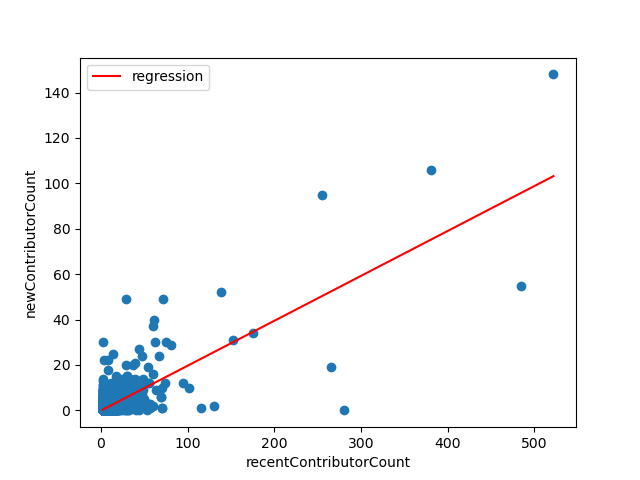
\includegraphics[width=\textwidth]{../experiment/data_analysis/recentContributorCountRegression_linearScale}
            \caption{Échelle linéaire}
        \end{subfigure}%
        \begin{subfigure}[t]{0.5\textwidth}
            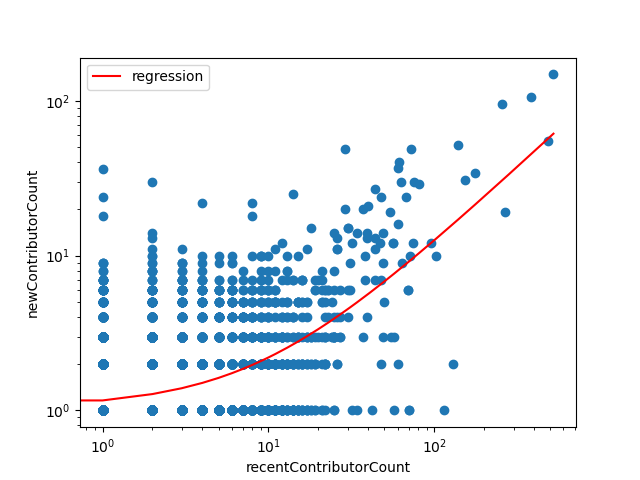
\includegraphics[width=\textwidth]{../experiment/data_analysis/recentContributorCountRegression_logScale}
            \caption{Échelle logarithmique}
        \end{subfigure}

        $\mathit{newContributorCount} = \mathit{recentContributorCount} * 0.11540180 + 1.04427117$\\($r^2 = 0.28318792$)

        Test d'homoscédasticité de White : $LM = 16280.789$ ($p = 0$)

        \caption{Nombre de nouveaux contributeurs en fonction du nombre de contributeurs récents uniques}
        \label{fig:contributorCount}
    \end{figure}

    Un premier modèle utilisant la méthode des moindres carrés ordinaires a été calculé, puis soumis à un test
    d'homoscédasticité de White ayant conclu, à l'inverse, à une forte hétéroscédasticité des données de la
    régression ($p = 0$). Cette hétéroscédasticité signifie que les données ont une variance fortement
    hétérogène au sein du problème, ce qui implique que la méthode OLS n'est pas la plus statistiquement
    efficace pour modéliser la relation entre les deux variables \parencite{GLS-2021}.

    Le modèle retenu a donc finalement été calculé par la méthode des moindres carrés généralisée (modèle
    \href{https://www.statsmodels.org/dev/generated/statsmodels.regression.linear_model.GLS.html}{GLS} du
    paque Python \texttt{statsmodel}), il suggère effectivement que plus le nombre de contributeurs récents
    d'un projet est élevé, plus son nombre de nouveaux contributeurs l'est aussi. Le coefficient de
    détermination $R^2 \approx 0.45$ du modèle indique que le nombre de contributeurs récents explique environ
    $45\%$ de la variation du nombre de nouveaux contributeurs, ce qui valide
    \hyperref[hyp:recentcontributorcount]{l'hypothèse H\ref*{hyp:recentcontributorcount}}, avec une taille
    d'effet tout de même modérée, voir faible.

    Ce résultat est aussi cohérent avec ceux de \textcite[p.~12-13,16]{signals-2019} qui observaient que le
    nombre de contributeurs uniques récents était positivement corrélé au nombre de \emph{tentatives} de
    contribution faites par de nouveaux contributeurs (mesuré par le nombre de \en{pull requests}). Là aussi
    de futures recherches pourraient s'intéresser à la causalité de cette relation. Tout ce que notre étude
    peut affirmer sur un éventuel lien de causalité est que, le nombre de contributeurs récents étant mesuré
    sur une période antécédente à celle sur laquelle est mesuré le nombre de nouveaux contributeurs, cette
    deuxième variable ne peut pas influencer la première, du moins tel que celles-ci ont été définies ici. Il
    reste à déterminer si une chaîne causale lie directement ces deux variables (si oui, laquelle) ou si elles
    ne sont liées que par un ancêtre causal commun (et si oui, lequel).

    \subsection{Lien entre le nombre de \en{commits} récents et le nombre de nouveaux contributeurs}

    Suivant la même approche que pour l'analyse du nombre de contributeurs récents, une première modélisation
    par régression linéaire suivant la méthode des moindres carrés ordinaires a d'abord été faite. Un test
    d'homoscédasticité de White a, là aussi, conclu à une forte hétéroscédasticité des données, c'est donc une
    régression linéaire utilisant la méthode des moindres carrés généralisée qui a été retenue
    (Fig.~\ref{fig:commitCount}).

    \begin{figure}[ht]
        \centering
        \begin{subfigure}[t]{0.5\textwidth}
            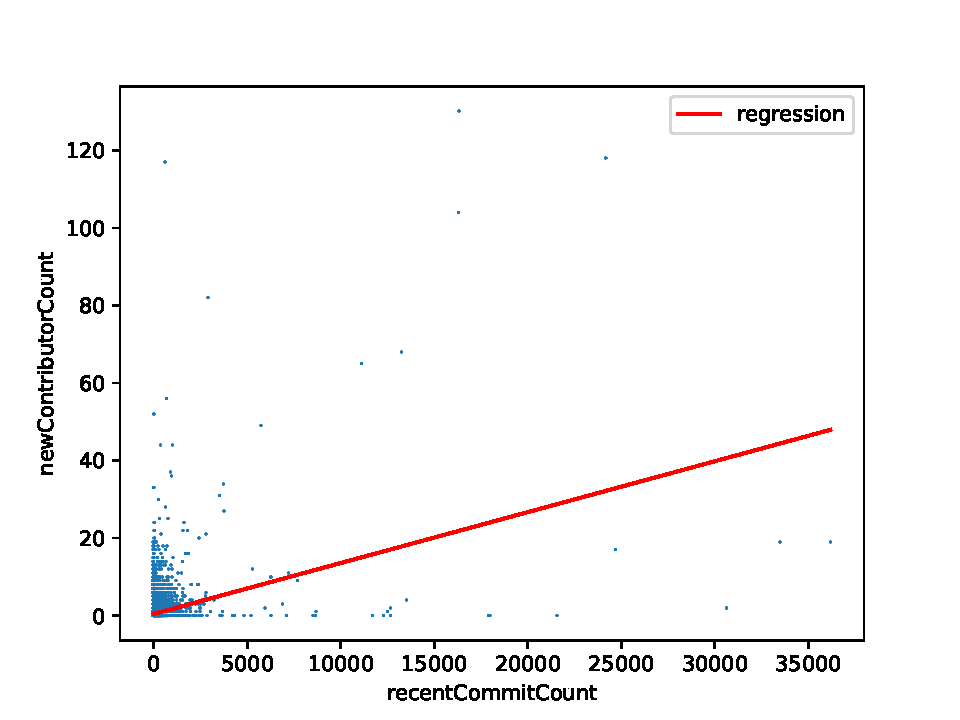
\includegraphics[width=\textwidth]{../experiment/data_analysis/recentCommitCountRegression_linearScale}
            \caption{Échelle linéaire}
        \end{subfigure}%
        \begin{subfigure}[t]{0.5\textwidth}
            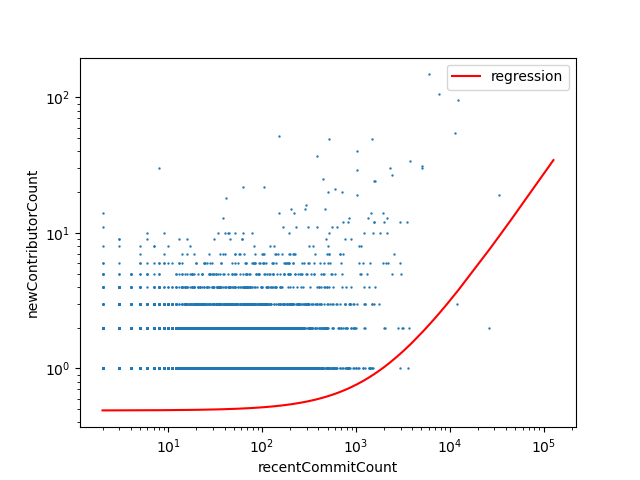
\includegraphics[width=\textwidth]{../experiment/data_analysis/recentCommitCountRegression_logScale}
            \caption{Échelle logarithmique}
        \end{subfigure}

        $\mathit{newContributorCount} = \mathit{recentCommitCount} \times 0.00026672041 + 0.48979364$\\($r^2 = 0.12749825$)

        Test d'homoscédasticité de White : $LM = 8150.885$ ($p = 0$)

        \caption{Nombre de nouveaux contributeurs en fonction du nombre de \emph{commits} récents}
        \label{fig:commitCount}
    \end{figure}
    \todo{TODO : retirer les formules dans toutes les figures de regression}

    Le modèle suggère ici aussi une corrélation positive entre le nombre de \en{commits} récents d'un projet
    et son nombre de nouveaux contributeurs, mais son coefficient de détermination est trop faible ($R^2
    \approx 0.10$) pour considérer que le modèle représente fidèlement des données du problème. Nous ne
    pouvons donc conclure à une relation entre ces deux variables et devons rejeter
    \hyperref[hyp:recentcommitcount]{l'hypothèse H\ref*{hyp:recentcommitcount}}.

    Ce résultat ne rejoint cette fois pas ceux de \textcite[p.~13,16]{signals-2019}, qui avaient là encore
    trouvé une corrélation positive entre le nombre de \en{commits} récents d'un projets et le nombre de
    tentatives de contribution faites par de nouveaux contributeurs. Cela pourrait potentiellement signifier
    que le nombre de \en{commits} récents d'un projet est un signal que les nouveaux contributeurs potentiels
    utilisent \emph{à tort} pour choisir un projet auquel essayer de contribuer. Nos résultats ne permettent
    pas de conclure qu'un grand nombre de \en{commits} récents, bien qu'il attire les nouveaux contributeurs,
    est un indicateur de l'accessibilité du projet pour ces nouveaux contributeurs.

    \section{Conclusion}

    Les problématiques liées au numérique prennent de plus en plus d'importance dans notre monde, la question
    du logiciel libre devient de ce fait un enjeu de société déterminant pour la transparence des
    technologies, l'ouverture de l'information et la collaboration international. Rendre disponible
    publiquement et gratuitement le code source et son processus de développement ne suffit cependant pas à le
    rendre réellement accessible, de nombreuses barrières existent pour les personnes souhaitant se
    familiariser avec les projets de logiciel libre et y contribuer. Ces barrières représentent même un frein
    pour les enseignants souhaitant introduire leurs étudiants à ce milieu, même lorsque ces enseignants lui
    sont eux-mêmes déjà familiers.

    Dans ce mémoire, nous avons commencé la construction d'un outil permettant aux enseignants de répondre à
    l'un de ces freins : la sélection de projets de logiciel libre réels susceptibles d'être un bon support de
    travaux pratiques. Ce travail préliminaire se base sur une littérature florissante d'identification des
    barrières aux contribution dans le logiciel libre, sa méthodologie s'inscrit quant à elle dans le domaine
    de l'analyse automatique des dépôts logiciels (\href{https://conf.researchr.org/series/msr}{\en{Mining
    Software Repositories}}).

    Par l'analyse de l'archive de Software Heritage, l'un des corpus de développement logiciel les plus
    représentatifs et exploitables dans un contexte de recherche, nous avons tenté de déterminer si trois
    signaux facilement observables pour un enseignant ou un nouveau contributeur sont prédictifs de la
    capacité d'un projet à suffisamment accompagner les nouveaux contributeurs pour leur permettre de mener
    leur première contribution à terme.

    Nos résultats suggèrent que la présence d'instructions de contribution au sein d'un projet (typiquement au
    travers d'un fichier \texttt{CONTRIBUTING.md}), ainsi que le nombre de contributeurs uniques ayant
    récemment contribué au projet, sont positivement corrélés au nombre de \emph{nouveaux} contributeurs étant
    parvenus à ajouter leur pierre à l'édifice. Nous n'avons en revanche pas trouvé de corrélation, positive
    ou négative, permettant d'affirmer que le nombre de \en{commits} récents au sein d'un projet était
    prédictif du nombre de nouveaux contributeurs allant au bout de leur contribution.

    Quelques précautions mériteraient cependant d'être prises dans l'interprétation de ces résultats. La
    limite la plus importante de ce travail est l'absence d'information permettant d'inférer un quelconque
    lien de causalité entre les éléments étudiés. Rien dans nos résultats ne nous permet par exemple de dire
    que la présence d'instructions de contribution \emph{améliore} l'accessibilité d'un projet de logiciel
    libre pour les nouveaux contributeurs, la corrélation que nous observons entre ces deux variables pourrait
    s'expliquer par le fait que les mainteneurs d'un projet qui ont tendance à efficacement guider les
    nouveaux contributeurs ont aussi tendance à écrire des instructions de contribution. Par ailleurs,
    plusieurs propriétés statistiques des données collectées rendent difficile leur analyse. Nous avons tenté
    traiter ces difficultés au mieux de nos capacités, mais une étude et une préparation plus rigoureuse des
    données pourraient, au mieux, améliorer la fiabilité des conclusions que nous en avons tiré, ou au pire,
    les invalider.

    Les perspectives de recherche concernant l'accessibilité des projets de logiciel libre sont encore
    nombreuses, le sujet étant à la fois très changeant et relativement nouveau, la littérature existe mais
    est encore très qualitative. De futures études quantitatives pourraient s'intéresser aux éventuels
    mécanismes causaux responsables de l'accessibilité observée des projets. Le domaine de l'analyse
    automatique des dépôts logiciels pose encore beaucoup de questions intéressantes, l'archive de Software
    Heritage par exemple apporte une nouvelle méthode d'observation particulièrement puissante, mais celle-ci
    est encore jeune et peu d'étude se consacrent aux bénéfices et limites de ce qu'elle peut apporter à la
    science. Enfin, si nos résultats suggèrent que la présence d'instructions de contribution ainsi que le
    nombre de contributeurs uniques récents sont de bons indicateurs à observer pour un enseignant souhaitant
    trouver un projet sur lequel faire travailler ses étudiants, de futures recherches mériteraient d'être
    conduites afin de déterminer si cette accessibilité se traduit effectivement dans la qualité de
    l'apprentissage, ou si le contexte est trop différent pour que les étudiants soient réduit à la catégorie
    générique des nouveaux contributeurs.

    \todo{TODO : réduire le nombre d'URL dans la biblio (garder seulement le doi) et voir s'il n'y a pas
    d'autres simplifications possibles, retirer les backrefs par exemple}
    \printbibliography[heading=bibintoc]
\end{document}
